%
% Author: Peter Schüller <schueller.p@gmail.com> 2014
%
% This work is licensed under a Creative Commons
% Attribution-NonCommercial-ShareAlike 4.0
% International License. (CC BY-NC-SA)
%
\documentclass[ignoreframetext,envcountsect]{beamer}

\usepackage{etex} % fix some out-of-resource errors of latex
\usepackage{graphicx}
\graphicspath{{figures/}}
\usepackage{url} % for comfortable url displaying
\usepackage{hyperref} % for making links/urls clickable
\usepackage{listings} % for displaying source code
\lstset{tabsize=2,showspaces=false,showstringspaces=false}
\usepackage{tikz} % the pgf / tikz drawing package
\usepackage{color}
\usetikzlibrary{shapes,arrows,backgrounds,automata,%
matrix,patterns,arrows,decorations.pathmorphing,decorations.pathreplacing,%
positioning,fit,calc,decorations.text,shadows%
}

\beamertemplatenavigationsymbolsempty

% put frame number on each slide
\setbeamertemplate{footline}{\hfill\mbox{\quad\insertframenumber$_{\big.}$\quad}}

% speed nop via if, show per default
\newif\ifsnop\snoptrue
% use \snopfalse to hide every slide after that
% and then \snoptrue to show every slide afterwards

% nop via if, hide per default
\newif\ifnop\nopfalse

% comfort macros
\newcommand{\bi}{\begin{itemize}}
\newcommand{\ei}{\end{itemize}}
\newcommand{\cemph}[1]{{\color{red}#1}}

% acknowledgement
\newcommand{\acknowledgegitolite}[0]{%
  \begin{tikzpicture}[overlay,remember picture]%
    \node[anchor=south east] at (current page.south east) {%
    \scriptsize \begin{tabular}{@{}r@{}}image from `Git Concepts Simplified'\\ by Sitaram Chamarty\end{tabular}};
  \end{tikzpicture}}

\pagestyle{empty}
\begin{document}

\ifsnop
\begin{frame}
\vfill
\centerline{\Huge Version Control with Git}
\medskip
\centerline{\huge and why it is important}
\medskip
\centerline{\huge for Free Software}
\vfill
\centerline{\Large Yrd.~Doç.~Peter Schüller}
\smallskip
\centerline{\Large Marmara University}
\smallskip
\centerline{\Large Computer Engineering}
\vfill
\centerline{\begin{minipage}{0.85\textwidth}\scriptsize
	This work is licensed under a Creative Commons
	Attribution-NonCommercial-ShareAlike 4.0
	International License. (CC BY-NC-SA)
	\end{minipage}}
\vfill
\end{frame}
\fi

\pagestyle{plain}

\ifsnop
\begin{frame}
\frametitle{Diffs}
\bi
\item
  Diff: Compares two files and tries to find only the changes.
  \medskip

  {\tt \$ diff <file1> <file2>}
\bigskip
\item
  Diffs are used to show how source code changes:
  \bi
  \item shows what changed
  \item shows 1,2,3 lines above and below (called `context')
  \ei
\ei
\end{frame}
\fi

\lstset{language={}}

\ifsnop
\begin{frame}
\scriptsize
\begin{tabular}{c@{\qquad}c}
\cemph{\tt file1} & \cemph{\tt file2} \\
\lstinputlisting{figures/file1} &
\lstinputlisting{figures/file2}
\end{tabular}
\medskip

\small
\begin{tabular}{c}
\cemph{{\tt \$ diff -c file1 file2}} \\
\lstinputlisting{figures/diffdemo.txt}
\end{tabular}
\end{frame}
\fi


\ifsnop
\begin{frame}
\frametitle{Diffs for tracking changes of Sourcecode}
With diffs we can
\medskip
\bi
\item \cemph{show differences} between versions.
\medskip
\item \cemph{recover old versions} by applying the reverse of the diff

  (a diff stores old and new version of everything that changes)
\medskip
\item \cemph{merge} changes if two people worked on the same file: 
  \bi
  \item
    a diff stores not only line numbers but also context

    $\Rightarrow$ apply the change in the nearest similar context
  \item
    if the same lines are changed, this is called \cemph{conflict}
  \item
    if no same lines are changed, automatic merge works well!
  \ei
\medskip
\item
  Note:
  \bi
  \item git does \emph{not} store versions using Diffs (it is more clever)
  \item git \emph{shows} version differences using Diffs (it is user friendly)
  \ei
\ei
\end{frame}
\fi


\ifsnop
\begin{frame}
\frametitle{Git Repository}
\bi
\vfill
\item
  Commit = a collection of diffs
\item
  Repository = an acyclic graph of commits
\item
  A commit points to one or more previous commits (history)
\item
  There might be several root nodes (branches)
\vfill
\item
  Committing a change = creating a new commit with parent
\ei
\centerline{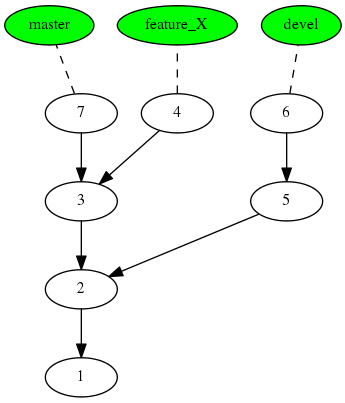
\includegraphics[scale=0.4]{threebranches}}
\acknowledgegitolite
\end{frame}
\fi


\ifsnop
\begin{frame}
\frametitle{Merging (master gets everything from feature\_X)}
\bi
\item
  We combine two branches: new commit with two parents
\ei
\centerline{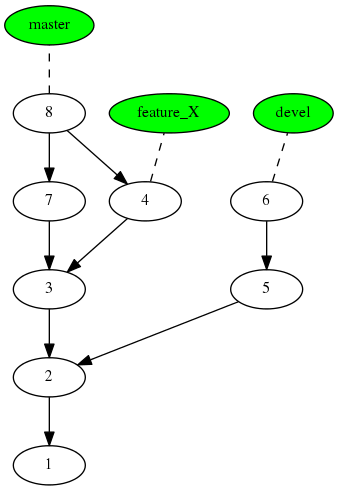
\includegraphics[scale=0.4]{threebranchesmerged}}
\acknowledgegitolite
\end{frame}
\fi


\ifsnop
\begin{frame}
\frametitle{Merging (feature\_X gets everything from master)}
\centerline{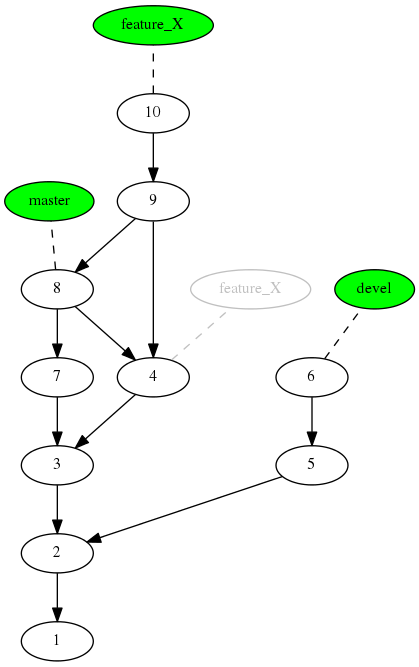
\includegraphics[scale=0.35]{threebranchesbackmerged}}
\acknowledgegitolite
\end{frame}
\fi


\ifsnop
\begin{frame}
\frametitle{Remotes - fetch/clone/pull/push}
\bi
\item A `remote' is a \cemph{link to another git repository}
\vfill
\item
  We can \cemph{fetch} from that repository  = get commits
\vfill
\item
  We can \cemph{clone} a repository
  
  clone = fetch + setup tracking local $\Leftrightarrow$ remote branch
\vfill
\item
  We can \cemph{pull} if we are on a tracked branch

  `pull' = `fetch' plus `merge' the tracked branch
\vfill
\item
  We might be allowed to \cemph{push} to a repository = send commits
  
  (git forbids destructive pushes without {\tt -force})
\vfill
\item
  Usually: we clone once, then we pull and push
\ei
\end{frame}
\fi


\ifsnop
\begin{frame}
\frametitle{Remotes, HEAD, and Tags}
\bi
\item
  The currently checked-out commit is called HEAD
\item
  Every commit can have a special name, a Tag (e.g., "v2.3.4")
\item
  Remotes are another kind of special name for commits.
\ei
\centerline{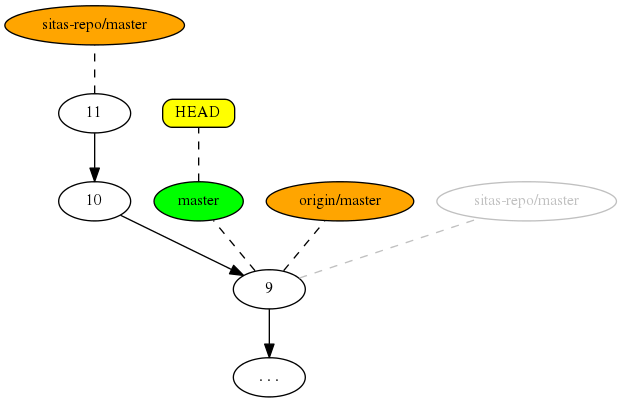
\includegraphics[scale=0.4]{remote}}
\acknowledgegitolite
\end{frame}
\fi


\ifsnop
\begin{frame}
\frametitle{Remotes - We do some work on {\tt master}}
\centerline{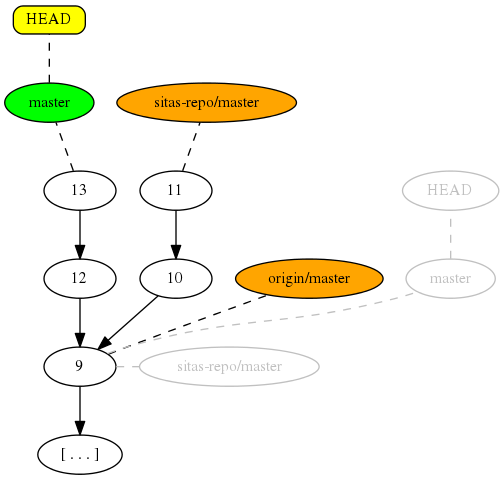
\includegraphics[scale=0.4]{remotemergedfetched}}
We can push to origin but not to sitas-repo (would lose 10 and 11).
\acknowledgegitolite
\end{frame}
\fi

\ifsnop
\begin{frame}
\frametitle{Remotes after {\tt \$ git merge sitas-repo/master}}
\centerline{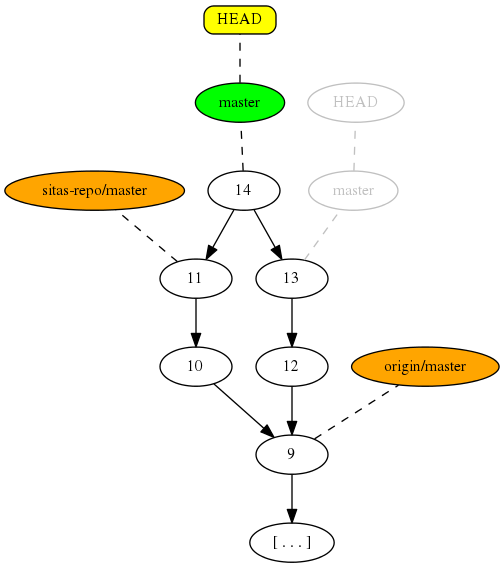
\includegraphics[scale=0.4]{remotemergedfetchedmerged}}
\vspace*{-3em}
Now we could push to\\
origin and to sitas-repo.
\acknowledgegitolite
\end{frame}
\fi


\ifsnop
\begin{frame}
\frametitle{A partial history of Version Control versus git}
\bi
\item
  Manual version control: main.cpp, main.cpp.v1, main.cpp.v2
\item 
  CVS version control:
  \bi
  \item
    Every file has a version number.
  \item
    Branches are possible, merging is difficult.
  \ei
\item 
  SVN version control:
  \bi
  \item
    Repository has a single version number (good and bad).
  \item
    Branching by copying and merging diffs
     
    (Merge algorithms better than CVS, but worse than git.)
  \item
    Checkouts are big (everything exists twice).
  \ei
\item
  Common weaknesses of CVS/SVN:
  \bi
  \item
    No history is stored at the user

    $\Rightarrow$ we need internet, slow blame/log operations
  \item
    We cannot commit without fetch+merge:
    
    $\Rightarrow$ every commit potentially destroys our changes

    $\Rightarrow$ we need internet to save any changes
  \ei
\item
  (Weakness of git: partial checkouts.)
\ei
\end{frame}
\fi



\ifsnop
\begin{frame}
\frametitle{Cryptographic SHAs 160 bit commit hashes}
\bi
\item
  SHA = Secure Hash Algorithm
\item
  SHA \cemph{uniquely and globally} identifies software history
\item
  SHA is built from:
  \bi
  \item Current software content
  \item SHA of parent commit(s)
  \item Commit message
  \item Author name/email/timestamp
  \item Committer name/email/timestamp
  \ei
\item
  Big security- and architecture-advantage of Git!
\ei
\end{frame}
\fi


\ifsnop
\begin{frame}
\frametitle{How SHAs make Free Software safer}
\bi
\item
  SHA is cryptographically strong.
\item[$\Rightarrow$]
  We assume that nobody can create a commit that reproduces a certain SHA value.
\item[$\Rightarrow$]
  Manipulating sourcecode or sourcecode histories is impossible!
\medskip
\item
  This is important in Free Software:
  \bi
  \item Someone might want to add code to the Linux Kernel by injecting it into an old version.
  \smallskip
  \item They can try, but \ldots
  \item \ldots suddenly all SHAs will be wrong.
  \smallskip
  \item[$\Rightarrow$] Every kernel developer will notice (broken hashes).
  \smallskip
  \item[$\Rightarrow$] Nobody can modify (history of) Sourcecode unnoticed.
  \ei
\ei
\end{frame}
\fi

\ifsnop
\begin{frame}
\frametitle{Distributed Version Control}
\bi
\item
  Every repository contains the complete history of HEAD
\item
  Every repository can fetch from every other repository
\item
  `Copied' history is handled correctly because of SHA!
\item
  Data is never duplicated because of SHA.
\item
  If one server crashes, every client is a backup.
\item
  Data-\cemph{deduplication} (in pack-files):
  \bi
  \item duplicate files are stored once
	\item history is stored efficiently
  \ei
\item
  Nobody needs to trust anybody, as long as SHA is safe.
\ei
\end{frame}
\fi


\ifsnop
\begin{frame}
\frametitle{Software Tools}
\bi
\item
  Linux/MacOs/Windows Shell:
  \bi
  \item General: {\tt \$ git <subcommand> --help}
  \item {\tt \$ git init}
  \item {\tt \$ git \{add|rm|blame\} <file> }
  \item {\tt \$ git \{commit|status|diff\} }
  \item {\tt \$ git \{clone|fetch|pull|push\} }
  \item {\tt \$ git remote }
  \ei
\item
  Linux/MacOs/Windows GUIs:
  \bi
  \item View History: gitk
    \bi
    \item View branches, tags, remotes
    \item Find SHAs
    \ei
  \item Commit comfortably: git-cola (Linux/Mac) / Git GUI (Win)
    \bi
    \item Commit a part of your changes
    \item Undo a part of your changes
    \ei
  \ei
\item
  Many other tools support git! (Eclipse, ... plugins)
\ei
\end{frame}
\fi


\ifsnop
\begin{frame}
\frametitle{Demo}
\bi
\item Setup SSH Keys %(note to self: careful!)
\item New repo + send to bitbucket (or local):
  \bi
  \item {\tt \$ git init}
  \item {\tt \$ git \{status|add\}} or {\tt \$ git-cola}
  \item {\tt \$ git push <remotename> <branchname>}
  \ei
\item Clone repo
  \bi
  \item {\tt \$ git clone}
  \item make changes, commit, push
  \ei
\item Pull {\tt \$ git fetch}
\item Provoke Conflict \& view History {\tt \$ gitk}
\ei
%\centerline{\scriptsize (note to self: {\tt urxvt -bg \{lightgreen|lightred\}})}
%\centerline{\scriptsize (note to self: {\tt urxvt -fn "xft:Bitstream Vera Sans Mono:pixelsize=15"})}
\end{frame}
\fi



\ifsnop
\begin{frame}
\frametitle{Free Software Workflow}
\bi
\item You find a cool software that is open source.
\item You use it.
\item You find a bug, or you want to add something.
\item You think you can fix the bug or improve the software.
\item What can you do?
\pause
\item If the software is in github/bitbucket it is very easy!
\item You \cemph{fork} the sourcecode, change it, and make a \cemph{pull request}.
\ei

\medskip
Fork:
\bi
\item Your private copy of the complete repository in your account.
\item You can do whatever you think, it is safe for everyone.
\item Nobody must do anything (give permissions, etc.) for forking.
\ei
\end{frame}
\fi

\ifsnop
\begin{frame}
\frametitle{Pull request}
``Select some of your changes
and ask the original software maintainers
to \cemph{re-integrate} these changes into the source code.''
\medskip

Maintainers can
\bi
\item discuss the pull request with you and ask for improvements
  
  $\Rightarrow$ code formatting guidelines

  $\Rightarrow$ comments/documentation

  $\Rightarrow$ unrelated changes in same commit / bad commit messages
\item reject the pull request

  $\Rightarrow$ bad quality, or undesired/dangerous feature
\item accept the pull request

  $\Rightarrow$ your code becomes part of the official software
  
  $\Rightarrow$ your name and email address will be public in the git repo

  $\Rightarrow$ the next release contains your code $\Rightarrow$ you will be \cemph{famous!}
\ei
\end{frame}
\fi


\ifsnop
\begin{frame}
\frametitle{Motivation(s)}
\bi
\item Free Software improves if people \cemph{like you} contribute.
\medskip
\item Why is it motivating to contribute (without getting money)?
  \bi
  \item Your sourcecode in official Ubuntu/Debian/... - a good feeling!
  \item github.com shows your activity to the world
    (how much you contributed, including bug reports etc.)
  \item It can increase the change of getting a job.
  \item It can make your life as a researcher/programmer easier:
    \bi
    \item you create software
    \item but you need a change in another software for your software
    \item[$\Rightarrow$] if the change is generally useful
      $\Rightarrow$ create a clean pull request
      $\Rightarrow$ you help yourself and free software
    \ei
  \ei
\medskip
\item Earn money with free software by providing \cemph{service} to others.
  
  E.g.: training people to use it, configuring/extending it.
  
  That's a good thing, and can be a motivation!
\ei
\end{frame}
\fi


\ifsnop
\begin{frame}
\frametitle{Acknowledgements and Links}
\bi
\item
	`Got 15 Minutes and want to learn Git?'

	\centerline{
	\url{https://try.github.io/}
	}
\item
  `Git Concepts Simplified' by Sitaram Chamarty

  \centerline{
  \url{http://gitolite.com/gcs.html}
  }
\item
  There is a good git tutorial at

  \centerline{
  \url{http://git-scm.com/docs/gittutorial}
  }
\item
  There is a good guide for Git under Windows at

  \centerline{
  \url{http://nathanj.github.io/gitguide/}
  }
\item
  Get your own public free Git repository at
  
  \centerline{
  \url{http://github.com/} or \url{http://bitbucket.org/}
  }
\item
  Google/Yandex/StackOverflow is your friend if you need help.
\ei
\end{frame}
\fi

\end{document}

% vim:ts=2:noet:sw=2:
